\section{Theoretische Grundlagen}

\subsection{Standardmodell der Elementarteilchenphysik}

\begin{figure}[bh]
	\centering
	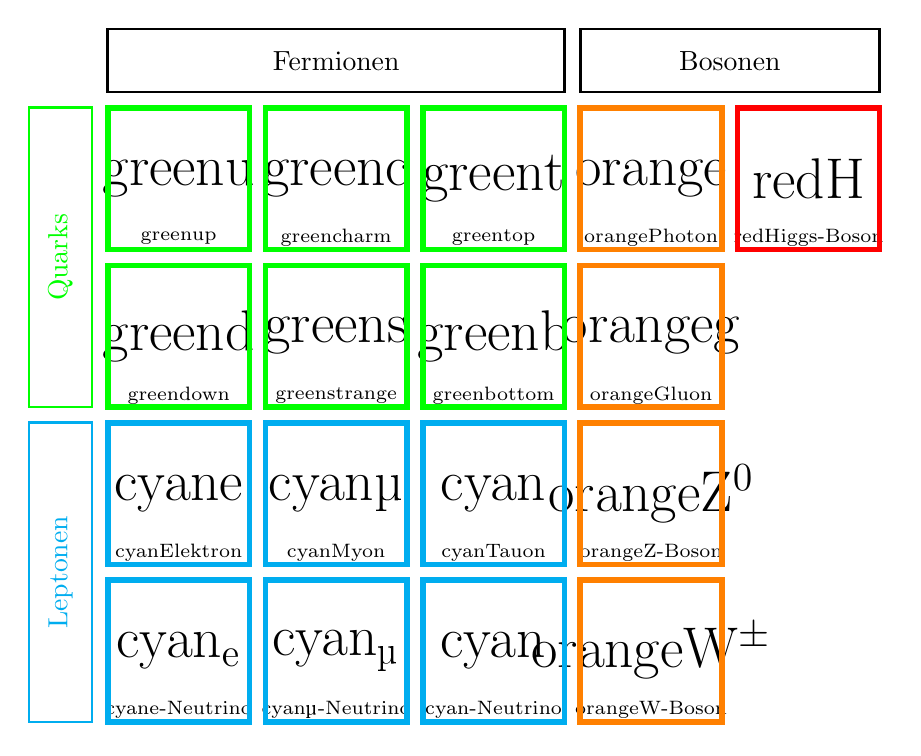
\begin{tikzpicture}
	\node at(0.9,-0.9){\huge\vcenterbf{green}{u}};
	\node at(2.9,-0.9){\huge\vcenterbf{green}{c}};
	\node at(4.9,-0.9){\huge\vcenterbf{green}{t}};
	\node at(0.9,-2.9){\huge\vcenterbf{green}{d}};
	\node at(2.9,-2.9){\huge\vcenterbf{green}{s}};
	\node at(4.9,-2.9){\huge\vcenterbf{green}{b}};
	\node at(0.9,-4.9){\huge\vcenterbf{cyan}{e}};
	\node at(2.9,-4.9){\huge\vcenterbf{cyan}{\textmu}};
	\node at(4.9,-4.9){\huge\vcenterbf{cyan}{\texttau}};
	\node at(0.9,-6.9){\huge \vcenterbf{cyan}{\textnu\textsubscript{e}}};
	\node at(2.9,-6.9){\huge \vcenterbf{cyan}{\textnu\textsubscript{\textmu}}};
	\node at(4.9,-6.9){\huge \vcenterbf{cyan}{\textnu\textsubscript{\texttau}}};
	\node at(6.9,-0.9){\huge\vcenterbf{orange}{\textgamma}};
	\node at(8.9,-0.9){\huge\vcenterbf{red}{H}};
	\node at(6.9,-2.9){\huge\vcenterbf{orange}{g}};
	\node at(6.9,-4.9){\huge\vcenterbf{orange}{Z\textsuperscript{0}}};
	\node at(6.9,-6.9){\huge \vcenterbf{orange}{W$^\pm$}};
	\node at(0.9,-1.65){\scriptsize\vcenternode{green}{up}};
	\node at(2.9,-1.65){\scriptsize\vcenternode{green}{charm}};
	\node at(4.9,-1.65){\scriptsize\vcenternode{green}{top}};
	\node at(0.9,-3.65){\scriptsize\vcenternode{green}{down}};
	\node at(2.9,-3.65){\scriptsize\vcenternode{green}{strange}};
	\node at(4.9,-3.65){\scriptsize\vcenternode{green}{bottom}};
	\node at(0.9,-5.65){\scriptsize\vcenternode{cyan}{Elektron}};
	\node at(2.9,-5.65){\scriptsize\vcenternode{cyan}{Myon}};
	\node at(4.9,-5.65){\scriptsize\vcenternode{cyan}{Tauon}};
	\node at(0.9,-7.65){\scriptsize \vcenternode{cyan}{e-Neutrino}};
	\node at(2.9,-7.65){\scriptsize \vcenternode{cyan}{\textmu-Neutrino}};
	\node at(4.9,-7.65){\scriptsize \vcenternode{cyan}{\texttau-Neutrino}};
	\node at(6.9,-1.65){\scriptsize\vcenternode{orange}{Photon}};
	\node at(8.9,-1.65){\scriptsize\vcenternode{red}{Higgs-Boson}};
	\node at(6.9,-3.65){\scriptsize\vcenternode{orange}{Gluon}};
	\node at(6.9,-5.65){\scriptsize\vcenternode{orange}{Z-Boson}};
	\node at(6.9,-7.65){\scriptsize \vcenternode{orange}{W-Boson}};
	
	\draw[line width=2,color=green] (0,0) rectangle (1.8,-1.8);
	\draw[line width=2,color=green] (2,0) rectangle (3.8,-1.8);
	\draw[line width=2,color=green] (4,0) rectangle (5.8,-1.8);
	\draw[line width=2,color=green] (0,-2) rectangle (1.8,-3.8);
	\draw[line width=2,color=green] (2,-2) rectangle (3.8,-3.8);
	\draw[line width=2,color=green] (4,-2) rectangle (5.8,-3.8);
	\draw[line width=2,color=cyan] (0,-4) rectangle (1.8,-5.8);
	\draw[line width=2,color=cyan] (2,-4) rectangle (3.8,-5.8);
	\draw[line width=2,color=cyan] (4,-4) rectangle (5.8,-5.8);
	\draw[line width=2,color=cyan] (0,-6) rectangle (1.8,-7.8);
	\draw[line width=2,color=cyan] (2,-6) rectangle (3.8,-7.8);
	\draw[line width=2,color=cyan] (4,-6) rectangle (5.8,-7.8);
	\draw[line width=2,color=orange] (6,0) rectangle (7.8,-1.8);
	\draw[line width=2,color=orange] (6,-2) rectangle (7.8,-3.8);
	\draw[line width=2,color=orange] (6,-4) rectangle (7.8,-5.8);
	\draw[line width=2,color=orange] (6,-6) rectangle (7.8,-7.8);
	\draw[line width=2,color=red] (8,0) rectangle (9.8,-1.8);
	
	\draw[line width=1,color=black] (0,1) rectangle (5.8,0.2);
	\draw[line width=1,color=black] (6,1) rectangle (9.8,0.2);
	\draw[line width=1,color=green] (-1,0) rectangle (-0.2,-3.8);
	\draw[line width=1,color=cyan] (-1,-4) rectangle (-0.2,-7.8);
	
	\node at(2.9,0.6){Fermionen};
	\node at(7.9,0.6){Bosonen};
	\node[rotate=90,color=green] at(-0.6,-1.9){Quarks};
	\node[rotate=90,color=cyan] at(-0.6,-5.9){Leptonen};
	
	
	\end{tikzpicture}
	\caption{Standardmodell der Elementarteilchenphysik}
	\label{fig:standardmodell}
\end{figure}

Das in Abbildung \ref{fig:standardmodell} dargestellte Standardmodell der Elementarteilchenphysik beschreibt die aktuellen Erkenntnisse der Teilchenphysik. Es beschreibt die uns bisher bekannten Elementarteilchen, sowie deren Wechselwirkungen mit Ausnahme der sehr schwachen Gravitation. Die Elementarteilchen lassen sich nach ihrem Spin in Fermionen und Bosonen einteilen, wobei die Teilchen mit halbzahligem Spin als Fermionen bezeichnet werden, während der Spin der Bosonen ganzzahlig ist.


\subsubsection{Wechselwirkungen}
Das Standardmodell beschreibt drei fundamentale Wechselwirkungen, die elektromagnetische Wechselwirkung, die schwache Wechselwirkung und die starke Wechselwirkung. Diese Wechselwirkungen werden durch den Austausch von Eichbosonen vermittelt. Die Eichbosonen und die Elementarteilchen, welche den Wechselwirkungen unterliegen werden in Abschnitt \ref{sec:elementarteilchen} eingeführt. Zu jeder Wechselwirkung existiert eine Ladung, die elektromagnetische Ladung, die schwache Ladung sowie die Farbladung der starken Wechselwirkung. Einer Wechselwirkung unterliegen nur Teilchen, die eine entsprechende Ladung tragen. Während die elektromagnetische Wechselwirkung eine unbegrenzte Reichweite hat, ist die Reichweite der schwachen und der starken Wechselwirkung kleiner als ein Atomkernradius. Die starke Wechselwirkung ermöglicht den Aufbau von Hadronen aus Quarks, welche als einige Teilchen der starken Wechselwirkung unterliegen, während die schwache Wechselwirkung für viele Zerfälle und Umwandlungen von Teilchen verantwortlich ist. Wechselwirkungen zwischen Atomen liegt die elektromagnetische Wechselwirkung zu Grunde.

\subsubsection{Elementarteilchen}\label{sec:elementarteilchen}
Fermionen und aus ihnen aufgebaute Teilchen werden als Materie bezeichnet. Die elementaren Fermionen, die Grundbausteine der Materie, lassen sich wiederum in Quarks und Leptonen einteilen. 
\paragraph{Quarks} Als Quarks werden die sechs elemntaren Fermionen bezeichnet, welche eine Farbladung tragen. Die elektromagnetische Ladung der oberen Quarks (up-, charm-, und top-Quark) beträgt $Q=\frac23$, wohingegen die unteren Quarks (down-, strange- und bottom-Quark) die Ladung $Q=\frac13$ tragen. Zu jedem Quark existiert ein Antiquark mit der entgegengesetzten Ladung ($Q_{\bar{q}}=-Q_q$).
\paragraph{Leptonen} Die übrigen elementaren Fermionen werden als Leptonen bezeichnet. Man unterscheidet hier zwischen den geladenen Leptonen (Elektron, Myon und Tauon) mit einer elektromagnetischen Ladung $Q=-1$ und den ungeladenen Leptonen, den sogenannten Neutrinos mit einer elektromagnetischen Ladung $Q=0$. Es lässt sich jedem geladenen Lepton ein dazugehöriges Neutrino zuordnen. Zu jedem Lepton existiert ein Antiteilchen. Die Antiteilchen der geladenen Leptonen haben jeweils die Ladung $Q=1$. Die Antineutrinos sind wie die Neutrinos neutral geladen.
\paragraph{Eichbosonen}
Die Bosonen lassen sich in Vektorbosonen (Spin $S=1$) und skalare Bosonen (Spin $S=0$) unterteilen. Die Vektorbosonen sind die Austauschteilchen der Wechselwirkungen, sogenannte Eichbosonen, während das einzige skalare Boson das Higgs-Boson ist. Die elektromagnetische Wechselwirkung wird über das Photon übertragen, das Gluon ist das Austauschteilchen der starken Wechselwirkung und die Eichbosonen der schwachen Wechselwirkung sind das geladene $W^\pm$- und das ungeladene $Z^0$-Boson.

\subsubsection{Elektroschwache Wechselwirkung}

Die elektroschwache Wechselwirkung ist eine vereinheitlichte Theorie der elektromagnetischen und der schwachen Wechselwirkung und vereint somit zwei der vier bekannten fundamentalen Wechselwirkungen. Mathematisch wird dabei eine $SU(2)$ und eine $U(1)$ Eichgruppe betrachtet. Erstere wird mit den drei W-Bosonen des schwachen Isospins identifiziert während letztere durch das B-Boson der schwachen Ladung beschrieben wird. Diese Bosonen sind dabei zunächst alle masselos. Die bekannten Austauschteilchen $\gamma$ und $W^{\pm}$, $Z_0$ der elektromagnetischen und schwachen Wechselwirkung entstehen durch die sogenannte Symmetriebrechung des Higgs-Mechanismus, sie sind eine Mischung der einzelnen Eichbosonen und sind wie folgt beschrieben:

\begin{align}
W^{\pm}=\frac{1}{\sqrt{2}}\cdot(W_1 \mp W_2)
\end{align}

\begin{align}
\begin{pmatrix}\gamma\\Z^{0}\end{pmatrix}=\begin{pmatrix}\cos(\Theta_W) \sin(\Theta_W)\\\sin(\Theta_W) \cos(\Theta_W)\end{pmatrix} \cdot \begin{pmatrix}B\\W_3\end{pmatrix}
\end{align}

wobei $\Theta_W$ den Weinbergwinkel bezeichnet, der das Mischungsverhältnis angibt. Er ist gegeben als $\Theta_W = 28,74$. Es lassen sich außerdem folgende Relationen für den Kosinus und den Sinus des Weinbergwinkels ableiten:

\begin{align}
\cos(\Theta_W) = \frac{M_W}{M_Z}
\end{align}

wobei $M_W$ und $M_Z$ für die Masse des W- bzw. $Z^{0}$-Bosons stehen, sowie

\begin{align}
\sin(\Theta_W)=\frac{e}{g}
\end{align}

wobei $e$ und $g$ die Kopplungskonstanten der elektromagnetischen und der schwachen Wechselwirkung bezeichnen.

\subsection{Das Z\textsuperscript0-Boson}

Wie in Abschnitt \ref{sec:elementarteilchen} erwähnt, existieren drei Eichbosonen der schwachen Wechselwirkung. Die geladenen Eichbosonen $W^+$ und $W^-$ spielen beispielsweise eine wichtige Rolle für den $\beta$-Zerfall. Ein Neutron zerfällt in ein Proton, in dem sich ein down-Quark unter Aussendung eines $W^-$ in einen up-Quark umwandelt. Das $W^-$ zerfällt daraufhin in ein Elektron und ein Anti-Elektron-Neutrino. Das $W^\pm$ erzeugt also Übergänge mit Ladungsänderung.\\

Es sind jedoch auch neutrale, ladungserhaltende Prozesse in der schwachen Wechselwirkung möglich. Diese werden durch den Austausch eines $Z^0$-Bosons durchgeführt. Das $Z^0$-Boson entsteht beispielsweise durch die Kollision von Elektronen und Positronen, den Antiteilchen des Elektrons mit einer Schwerpunktsenergie nahe der Masse des $Z^0$-Bosons. Anschließend zerfällt es in beliebige $f\bar{f}$-Paare, wobei $f$ für ein beliebiges Fermion und $\bar{f}$ für das dazugehörige Antiteilchen steht.

\subsection{e$^+$e$^-$-Prozesse}\label{sec:e+e-}

In diesem Versuch werden Daten von Elektron-Positron-Kollisionen ausgewertet. Bei dieser Kollision sind die folgenden verschiedenen Prozesse möglich.
\paragraph{Paarvernichtung und Erzeugung von Photonen}
Bei der Kollision von Elektron und Positron können diese sich annihilieren und dabei in zwei oder drei reelle Photonen zerfallen. Die Energie der Teilchen wird dabei vollständig an die Photonen übertragen. Dieser Prozess ist in Abbildung \ref{fig:feynmanphotonen} dargestellt. Bei diesem Prozess ist kein $Z^0$-Boson beteiligt, weshalb der Prozess in der Auswertung eliminiert werden muss.

\begin{figure}[b]
	\centering
	\begin{tikzpicture}
		\begin{feynman}
			\vertex (em) {$e^-$};
			\vertex [below right=of em](a);
			\vertex [below=of a](b);
			\vertex [below left=of b](ep){$e^+$};
			\vertex [above right=of a](p1){$\gamma$};
			\vertex [below right=of b](p2){$\gamma$};
			
			\diagram{
				(em)--[fermion](a)--[fermion](b)--[fermion](ep),
				(a)--[photon](p1),
				(b)--[photon](p2),
				};
		\end{feynman}
	\end{tikzpicture}
	\caption{Feynman-Graph der Erzeugung zweier Photonen}
	\label{fig:feynmanphotonen}
\end{figure}

\paragraph{Paarvernichtung und Erzeugung eines $Z^0$-Bosons}
Bei der Annihilation des Elektron-Positron-Paares kann ein virtuelles Photon und bei entsprechender Schwerpunktsenergie ein $Z^0$-Boson erzeugt werden. Dieses wiederum zerfällt nun in ein beliebiges $f\bar f$-Paar. In Abbildung \ref{fig:feynmanz0} ist dieser Prozess dargestellt.

\begin{figure}
	\centering
	\begin{tikzpicture}
	\begin{feynman}
	\vertex (em) {$e^-$};
	\vertex [below right=of em](a);
	\vertex [right=of a](b);
	\vertex [below left=of a](ep){$e^+$};
	\vertex [above right=of b](f1){$\bar f$};
	\vertex [below right=of b](f2){$f$};
	
	\diagram{
		(em)--[fermion](a)--[fermion](ep),
		(a)--[boson,edge label={$\gamma, Z^0$}](b),
		(f1)--[fermion](b)--[fermion](f2),
	};
	\end{feynman}
	\end{tikzpicture}
	\caption{Feynman-Graph der Erzeugung eines Z\textsuperscript0-Bosons}
	\label{fig:feynmanz0}
\end{figure}

\paragraph{Bhabha-Streuung}
Die Bhabha-Streuung beschreibt den Prozess $e^+e^-\rightarrow e^+e^-$. Zusätzlich zur oben beschrieben Annihilation muss hier noch die elastische Streuung von Elektron und Positron unter Austausch eines virtuellen Photons oder $Z^0$-Bosons betrachtet werden. Die Bhabha-Streuung ist in Abbildung \ref{fig:feynmanbhabha} dargestellt.


\begin{figure}
	\centering
	\begin{tikzpicture}
		\begin{feynman}
		\vertex (ep) {$e^+$};
		\vertex [below right=of ep](a);
		\vertex [right=of a](b);
		\vertex [below left=of a](em){$e^-$};
		\vertex [above right=of b](f1){$e^+$};
		\vertex [below right=of b](f2){$e^-$};
		
		\diagram{
			(ep)--[fermion](a)--[fermion](em),
			(a)--[boson,edge label={$\gamma, Z^0$}](b),
			(f1)--[fermion](b)--[fermion](f2),
		};
		\end{feynman}
	\end{tikzpicture}
	\begin{tikzpicture}
		\begin{feynman}
		\vertex (ep) {$e^+$};
		\vertex [below right=of ep](a);
		\vertex [below=of a](b);
		\vertex [below left=of b](em){$e^-$};
		\vertex [above right=of a](f1){$e^+$};
		\vertex [below right=of b](f2){$e^-$};
		
		\diagram{
			(f1)--[fermion](a)--[fermion](ep),
			(a)--[boson,edge label={$\gamma, Z^0$}](b),
			(em)--[fermion](b)--[fermion](f2),
		};
		\end{feynman}
	\end{tikzpicture}
	\caption[Feynman-Graphen der Bhabha-Streuung]{Feynman-Graphen der Bhabha-Streuung (links: s-Kanal; rechts: t-Kanal)}
	\label{fig:feynmanbhabha}
\end{figure}

\paragraph{Inelastische Streuung}
Bei der inelastischen Streuung werden zwei virtuelle Photonen ausgesendet, welche anschließend durch Interaktion ein Hadron erzeugen. Der Prozess der inelastischen Streuung wird in Abbildung \ref{fig:feynmaninelastisch} dargestellt. Bei diesem Prozess ist kein $Z^0$-Boson beteiligt, weshalb der Prozess in der Auswertung eliminiert werden muss.

\begin{figure}
	\centering
	\begin{tikzpicture}
	\begin{feynman}
	\vertex (em) {$e^-$};
	\vertex [below right=of em](a);
	\vertex [below right=of a](p);
	\vertex [below left=of p](b);
	\vertex [below left=of b](ep){$e^+$};
	\vertex [right=of p](h){$h$};
	
	\diagram{
		(em)--[fermion](a)--[fermion](b)--[fermion](ep),
		(a)--[photon,edge label=$\gamma$](p),
		(b)--[photon,edge label'=$\gamma$](p),
		(p)--(h),
	};
	\end{feynman}
	\end{tikzpicture}
	\caption{Feynman-Graph der inelastischen Streuung}
	\label{fig:feynmaninelastisch}
\end{figure}

\subsection{Z\textsuperscript0-Resonanz}

Die Prozesse, welche die Erzeugung eines $Z^0$-Bosons beinhalten sind jeweils nur im Bereich um die Masse des $Z^0$-Bosons möglich. Durch Untersuchung dieser Prozesse bei unterschiedlichen Schwerpunktsenergien rund um die erwartete Masse des $Z^0$-Bosons lässt sich nun die genaue Masse sowie die Zerfallsbreite des $Z^0$-Bosons bestimmen. Erwartet wird ein Resonanzmaximum des Wirkungsquerschnitts bei der Masse $M_Z$ des $Z^0$-Bosons.

\subsubsection{Bhabha-Streuung}\label{sec:bhabha}

Wie bereits in Abschnitt \ref{sec:e+e-} beschrieben, tragen zwei Feynman-Graphen zur Bhabha-Streuung bei (siehe Abbildung \ref{fig:feynmanbhabha}). Der s-Kanal beschreibt den Beitrag des Vernichtungsprozesses, während der t-Kanal Streuprozesse beschreibt. Für die Messung der Zerfallsbreite des $Z^0$-Bosons ist also nur der s-Kanal relevant. Unterscheiden lassen sich die unterschiedlichen Prozesse am Streuwinkel $\theta$ zwischen dem einlaufenden und dem auslaufenden Elektron. Für große Winkel dominiert der s-Kanal, für kleine Winkel der t-Kanal. Die Winkelabhängigkeit des Wirkungsquerschnitts wird durch folgende Formel beschrieben:
\begin{align}
	\del[\sigma]{\Omega}&=s\cdot\left(1+\cos^2\theta\right)+t\cdot\left(1-\cos\theta\right)^{-2}\text{.}\label{eq:stkanal}
\end{align}

\begin{figure}
	\centering
	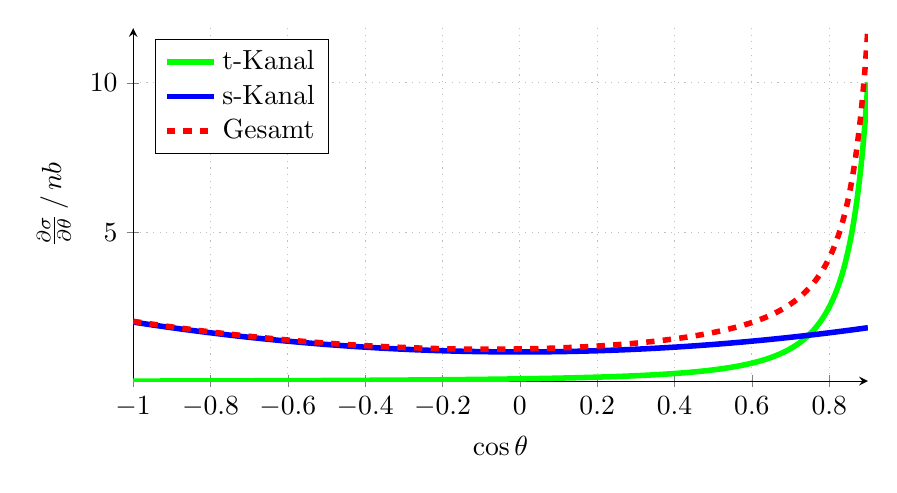
\begin{tikzpicture}
	\begin{axis}[
	width=0.9\textwidth,
	height=0.5\textwidth,
	axis lines=left, 
	xlabel=$\cos\theta$, 
	ylabel=$\frac{\partial \sigma}{\partial \theta}\,/\,\si{nb}$,
	ymajorgrids=true,
	xmajorgrids=true,
	grid style=dotted,
	legend pos=north west
	]
	\addplot[domain=-1:0.9,samples=1000,color=green,line width=2]
	{0.1*(1-x)^(-2)};
	\addlegendentry{t-Kanal};
	\addplot[domain=-1:0.9,samples=1000,color=blue,line width=2]
	{1*(1+x^2)};
	\addlegendentry{s-Kanal};
	\addplot[domain=-1:0.9,samples=1000,color=red,line width=2,style=dashed]
	{1*(1+x^2)+0.1*(1-x)^(-2)};
	\addlegendentry{Gesamt};
	\end{axis}
	\end{tikzpicture}
	\caption[Bhabha-Wirkungsquerschnitt für t-Kanal und s-Kanal]{Bhabha-Wirkungsquerschnitt für t-Kanal und s-Kanal.}
	\label{fig:winkelbhabhatheorie}
\end{figure}

\subsubsection{Annihilation in Fermionenpaare}
Die Paarvernichtung mit anschließendem Zerfall in ein $f\bar f$-Paar ist durch ein Photon oder ein $Z^0$-Boson möglich. Relevant für diesen Versuch ist nur der Zerfall durch das $Z^0$-Boson. Der Wirkungsquerschnitt in Abhängigkeit der Schwerpunktsenergie $E=\sqrt{s}$ ist gegeben durch eine Breit-Wigner-Verteilung:
\begin{align}
	\sigma_f(s)&=\frac{12\pi}{M_Z^2}\frac{s\Gamma_e\Gamma_f}{\left(s-M_Z^2\right)^2+\left(s\frac{\Gamma_Z}{M_z}\right)^2}\text{.}
\end{align}
Hierbei beschreibt $\Gamma_e$ die Zerfallsbreite des Elektrons, $\Gamma_f$ die Zerfallsbreite des Fermions und $\Gamma_Z$ die Gesamtbreite.

\subsubsection{Berechnung der Zerfallsbreiten}\label{sec:partialbreiten}

Die Partialbreiten der Zerfallskanäle berechnen sich nach \cite{anleitungalt} folgendermaßen:

\begin{align}
	\Gamma_f&=\frac{N_c^f\sqrt2}{12\pi}\cdot G_FM_Z^3\left(\left(g_v^f\right)^2+\left(g_A^f\right)^2\right)\label{eq:partialbreiten}
\end{align}
mit \cite{anleitungalt,nakamura}:
\begin{alignat}{2}
	&N_c^f&&=
	\begin{cases}
		1&\text{für } f\in\{e, \mu, \tau, \nu_e, \nu_\mu, \nu_\tau\}\\
		3&\text{für } f\in\{u, d, c, s, b\}
	\end{cases}\text{,}\\
	&G_F&&=(1,66370\pm0,00010)\cdot10^{-5}\,\si{GeV^{-2}}\text{,}\\
	&M_Z&&=(91,188\pm0,002)\,\si{GeV}\text{,}\\
	&g_v^f&&=I_3^f-2Q_f\sin^2\theta_W\text{,}\\
	&g_A^f&&=I_3^f\text{,}\\
	&I_3^f&&=
	\begin{cases}
		-\frac12&\text{für } f\in\{e, \mu, \tau, d, s, b\}\\
		\frac12&\text{für } f\in\{\nu_e, \nu_\mu, \nu_\tau, u, c\}
	\end{cases}\text{,}\\
	&Q_f&&=
	\begin{cases}
		-1&\text{für } f\in\{e, \mu, \tau\}\\
		-\frac13&\text{für } f\in\{d, s, b\}\\
		0&\text{für } f\in\{\nu_e, \nu_\mu, \nu_\tau\}\\
		\frac23&\text{für } f\in\{u, c\}
	\end{cases}\text{,}\\
	&\sin^2\theta_W&&=0,23116\pm0,00013\text{.}
\end{alignat}
Der Zerfall in $\tau\bar\tau$ ist aufgrund der hohen Masse des Top-Quarks nicht möglich.\\

Aus Gleichung \ref{eq:partialbreiten} ergeben sich folgende Ergebnisse:
\begin{alignat}{3}
	&\Gamma_{e/\mu/\tau}&&=&(83,412\pm0,009)\,\si{MeV}\text{,}\label{eq:leptonenuniversalitaet}\\
	&\Gamma_{\nu_e/\nu_\mu/\nu_\tau}&&=&\,(165,884\pm0,011)\,\si{MeV}\text{,}\label{eq:neutrinos}\\
	&\Gamma_{d/s/b}&&=&(367,91\pm0,06)\,\si{MeV}\text{,}\\
	&\Gamma_{u/c}&&=&(285,43\pm0,07)\,\si{MeV}\text{.}
\end{alignat}
Daraus lassen sich nun die gesamte Zerfallsbreite $\Gamma_Z$, die hadronische Zerfallsbreite $\Gamma_q$, die geladene leptonische Zerfallsbreite $\Gamma_l$ und die Neutrino-Zerfallsbreite $\Gamma_\nu$ zu folgenden Werten bestimmen:
\begin{alignat}{3}
	&\Gamma_Z&&=&(2422,5\pm0,2)\,\si{MeV}\text{,}\\
	&\Gamma_q&&=&\,(1674,59\pm0,19)\,\si{MeV}\text{,}\\
	&\Gamma_l&&=&(250,24\pm0,03)\,\si{MeV}\text{,}\\
	&\Gamma_\nu&&=&(497,65\pm0,03)\,\si{MeV}\text{.}
\end{alignat}

Der Wirkungsquerschnitt $\sigma_f$ zur Erzeugung eines $f\bar{f}$-Paars bei der Schwerpunktenergie $\sqrt{s}$ ist gegeben durch:
\begin{align}
	\sigma_f&=\frac{12\pi}{M_Z^2}\frac{s\Gamma_e\Gamma_f}{\left(s-M_Z^2\right)^2+\left(s\frac{\Gamma_Z}{M_Z}\right)^2}
\end{align}
und ergibt sich am Resonanzmaximum ($\sqrt{s}=M_z$) zu
\begin{align}
	\sigma_f^\text{Peak}&=\frac{12\pi}{M_Z^2}\frac{\Gamma_e}{\Gamma_Z}\frac{\Gamma_f}{\Gamma_Z}\text{.}
\end{align}

\begin{figure}
	\centering
	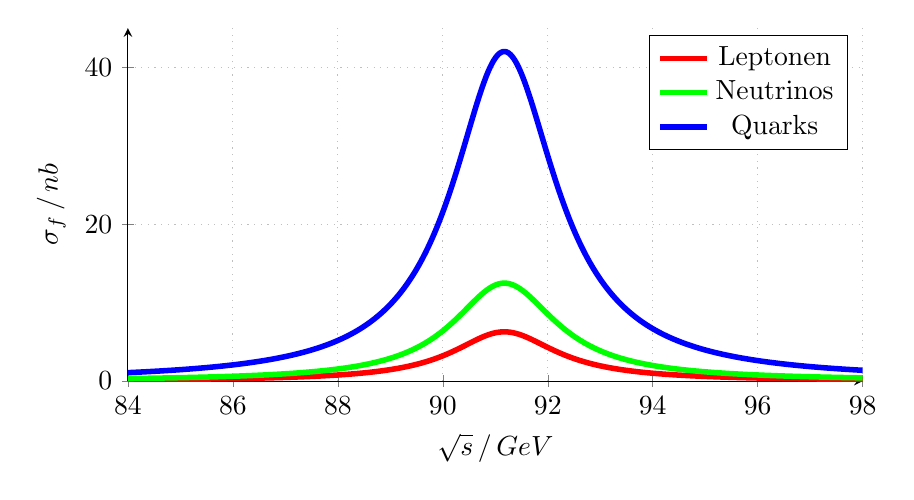
\begin{tikzpicture}
		\begin{axis}[
			width=0.9\textwidth,
			height=0.5\textwidth,
			axis lines=left, 
			xlabel=$\sqrt{s}\,/\,\si{GeV}$, 
			ylabel=$\sigma_f\,/\,\si{nb}$,
			ymajorgrids=true,
			xmajorgrids=true,
			grid style=dotted,
			ymin=0,ymax=45,
			xmin=84,xmax=98
		]
			\addplot[domain=80:100,samples=1000,color=red,line width=2]
			{0.3894*10^6*12*3.14159265359/(91.188^2)*x^2*0.083412*0.25024/((x^2-91.188^2)^2+x^4*(2.4225/91.188)^2)};
			\addlegendentry{Leptonen};
			\addplot[domain=80:100,samples=1000,color=green,line width=2]
			{0.3894*10^6*12*3.14159265359/(91.188^2)*x^2*0.083412*0.49765/((x^2-91.188^2)^2+x^4*(2.4225/91.188)^2)};
			\addlegendentry{Neutrinos};
			\addplot[domain=80:100,samples=1000,color=blue,line width=2]
			{0.3894*10^6*12*3.14159265359/(91.188^2)*x^2*0.083412*1.67459/((x^2-91.188^2)^2+x^4*(2.4225/91.188)^2)};
			\addlegendentry{Quarks};
		\end{axis}
	\end{tikzpicture}
	\caption[Partielle Wirkungsquerschnitte in Abhängigkeit der Schwerpunktsenergie]{Partielle Wirkungsquerschnitte in Abhängigkeit der Schwerpunktsenergie.}
	\label{fig:partialbreiten}
\end{figure}

Der Verlauf der Wirkungsquerschnitte für Leptonen, Neutrinos und Quarks ist in Abbildung \ref{fig:partialbreiten} dargestellt. Wir erhalten folgende partielle Wirkungsquerschnitte am Resonanzmaximum:
\begin{alignat}{3}
	&\sigma_q^\text{Peak}&&=&(42,022\pm0,010)\,\si{nb}\text{,}\\
	&\sigma_l^\text{Peak}&&=&\,(6,2794\pm0,0013)\,\si{nb}\text{,}\\
	&\sigma_{e/\mu/\tau}^\text{Peak}&&=&(2,0931\pm0,0006)\,\si{nb}\text{,}\\
	&\sigma_\nu^\text{Peak}&&=&(12,488\pm0,003)\,\si{nb}\text{,}
\end{alignat}
wobei $\sigma_{e/\mu/\tau}$ der Wirkungsquerschnitt eines einzelnen Leptons ist, während $\sigma_{l}$ der Wirkungsquerschnitt für alle geladenen Leptonen ist, so wie $\sigma_\nu$ der Wirkungsquerschnitt für alle Neutrinos ist.

\paragraph{Weitere Leptonengeneration} Falls der Zerfall des $Z^0$-Bosons in ein weiteres Lepton $x$ möglich ist, sind zwei zusätzliche Zerfallskanäle zu betrachten: $Z^0\rightarrow x\bar x$ und $Z^0\rightarrow \nu_x\bar{\nu}_x$. Nach Gleichung \ref{eq:partialbreiten} gilt dann:
\begin{alignat}{6}
	&\Gamma_x&&=\Gamma_{e/\mu/\tau}&&=&\,(83,412\pm\,0,009)\,\si{MeV}\text{,}\\
	&\Gamma_{\nu_x}&&=\Gamma_{\nu_e/\nu_\mu/\nu_\tau}&&=&\,(165,884\pm\,0,011)\,\si{MeV}\text{.}
\end{alignat}
Die relative Änderung der Zerfallsbreite beträgt also:
\begin{align}
	p&=\frac{\Delta\Gamma_Z}{\Gamma_Z}=\frac{\Gamma_x+\Gamma_{\nu_x}}{\Gamma_Z}=(10,2910\pm0,0010)\,\%\text{.}
\end{align}

\subsection{Vorwärts-Rückwärts-Asymmetrie}\label{sec:asymm}
Die Vorwärts-Rückwärts-Asymmetrie beschreibt den Unterschied der Wirkungsquerschnitte für Winkel $\theta>0$ und Winkel $\theta<0$. Sie ist definiert durch \cite{anleitungalt}:
\begin{align}
	A_{FB}&=\frac{\int\limits_0^1\del[\sigma]{\cos\theta}\mathrm d\cos\theta
		-\int\limits_{-1}^0\del[\sigma]{\cos\theta}\mathrm d\cos\theta}
	{\int\limits_0^1\del[\sigma]{\cos\theta}\mathrm d\cos\theta
		+\int\limits_{-1}^0\del[\sigma]{\cos\theta}\mathrm d\cos\theta}\text{.}\label{eq:asymm}
\end{align}

Nach der Born'schen Näherung gilt für den differentiellen Wirkungsquerschnitt der Reaktion $e^+e^-\rightarrow f\bar f$ \cite{anleitungalt}:
\begin{align}
	\diff[\sigma]{\Omega}&=\frac{\alpha^2\cdot N_c^f}{4s}\left(F_1(s)\cdot\left(1+\cos^2\theta\right)+2F_2(s)\cdot\cos\theta\right)\text{.}
\end{align}
Daraus ergibt sich für die Asymmetrie:
\begin{align}
	A_{FB}&=\frac34\frac{F_2}{F_1}\text{.}
\end{align}
Am Resonanzmaximum ergibt sich das zu \cite{anleitungalt}:
\begin{align}
	A_{FB}^{\mathrm{Peak}}&=3\left(1-4\sin^2\theta_W\right)^2\text{,}\label{eq:weinberg}
\end{align}
mit dem Weinbergwinkel $\theta_W$, welcher sich somit aus der Vorwärts-Rückwärts-Asymmetrie berechnen lässt.

\subsection{Strahlungskorrekturen}
Bei hohen Schwerpunktsenergien, wie sie in diesem Versuch vorkommen, kann die Born'sche Näherung nicht mehr ausreichend alle Effekte erklären. Deshalb müssen bei der Berechnung der Wirkungsquerschnitte Strahlungskorrekturen berücksichtigt werden. Zu berücksichtigen sind hier QED\footnote{\textbf Quanten\textbf Elektro\textbf Dynamik}-Korrekturen durch die elektroschwache Wechselwirkung, QCD\footnote{\textbf Quanten\textbf Chromo\textbf Dynamik}-Korrekturen durch die starke Wechselwirkung, sowie Korrekturen durch virtuelle Prozesse. Die Effekte, die zu diesen Korrekturen führen, sind im folgenden beschrieben und beispielhaft in Abbildung \ref{fig:korrekturen} dargestellt.

\paragraph{QED-Korrekturen}
QED-Korrekturen entstehen durch Bremsstrahlungseffekte, also ausgestrahlte Photonen aus dem Anfangs- oder Endzustand.

\paragraph{QCD-Korrekturen}
QCD-Korrekturen sind vergleichbar zu den QED-Korrekturen, der zugrunde liegende Effekt ist hier die Abstrahlung eines Gluons. Da Leptonen keine Gluonen abstrahlen können, kann dieser Effekt nur im Endzustand auftreten. Es können auch zwei Gluonen aus dem Endzustand abgestrahlt werden.

\paragraph{Virtuelle Korrekturen}
Virtuelle Korrekturen entstehen durch Prozesse, die den gleichen Anfangs- und Endzustand besitzen, wie der zugrundeliegende Prozess der Born'schen Näherung. Dies sind beispielsweise die Erzeugung und sofortige Vernichtung eines Fermionenpaars oder der Austausch eines Photons oder Z\textsuperscript0-Bosons zwischen zwei Start- oder Endteilchen.

%\begin{figure}
%	\centering
%	\subfigure[QED]{
%			\begin{tikzpicture}
%			\begin{feynman}
%			\vertex (em) {$e^-$};
%			\vertex [below right=of em](a);
%			\vertex [right=of a](b);
%			\vertex [below left=of a](c);
%			\vertex [below left=of c](ep){$e^+$};
%			\vertex [above right=of b](f1){$\bar f$};
%			\vertex [below right=of b](f2){$f$};
%			\vertex [below right=of c](g1){$\gamma$};
%			
%			\diagram{
%				(em)--[fermion](a)--(c)--[fermion](ep),
%				(c)--[photon](g1),
%				(a)--[boson,edge label={$\gamma, Z^0$}](b),
%				(f1)--[fermion](b)--[fermion](f2),
%			};
%			\end{feynman}
%			\end{tikzpicture}
%			\begin{tikzpicture}
%			\begin{feynman}
%			\vertex (em) {$e^-$};
%			\vertex [below right=of em](a);
%			\vertex [right=of a](b);
%			\vertex [below left=of a](ep){$e^+$};
%			\vertex [above right=of b](f1){$\bar f$};
%			\vertex [below right=of b](f2){$f$};
%			
%			\diagram{
%				(em)--[fermion](a)--[fermion](ep),
%				(a)--[boson,edge label={$\gamma, Z^0$}](b),
%				(f1)--[fermion](b)--[fermion](f2),
%			};
%			\end{feynman}
%			\end{tikzpicture}
%		}
%	\subfigure[QCD]{
%		}
%	\subfigure[virtuell]{
%		}
%	\caption{Strahlungskorrekturen durch \subref{sub:qed} QED, \subref{sub:qcd} QCD und \subref{sub:virtuell} virtuelle Prozesse}
%\end{figure}

\subsection{Teilchendetektoren}
Teilchendetektoren sind Detektoren, die dem Nachweis von Elementarteilchen und ihere Bestimmung dienen. Dabei werden die unterschiedlichen Eigenschaften wie Ladung, Masse und Art und Stärke der Wchselwirkung der verschiedenen Elementarteilchen ausgenutzt um eine Spur eindeutig einer Teilchensorte zuzuordnen. Da die einzelnen nachzuwesienden Teilchen sich in diesen Eigenschaften stark unterscheiden ist für eine vollständige Bestimmung eines Events meist eine Vielzahl verschiedener Detektoren notwendig. Im Folgenden soll ein grober Überblick über die in der Teilchenphysik geläufigsten und für diesen Versuch relevanten Detektoren gegeben werden.

\paragraph{Proportionalitätskammer}
Die Art der Wechselwirkung von Teilchen mit Materie, auf der Proportionalitätskammern beruhen, ist die Ionisation eines Gases. Proportionalitätslammern bestehen aus einem Gasvolumen, in dem sich ein positiv geladener Zähldraht befindet. Durchquert ein geladenes Teilchen ein Gasvolumen, kann es ein Elektron-Ionern-Paar bilden. Dieses sogenannte Primär-Elektron wandert zum Zähldraht und erhält durch das elektrische Feld ausreichend kinetische Energie um weitere Atome zu ionisieren, sodass es zu einem abrupten, starken Anstieg der Elektronenzahl im Gas kommt, die mit dem Zähldraht detektiert wird. 
Eine \textbf{Vieldrahtproportionalkammer} nutzt dieses Prinzip zur Ortsbestimmung in dem eine Vielzahl von Anodendrähten zwischen zwei Kathodenfl#ächen gespannt werden. Unabhängiges Auslesen dieser ermöglicht ine Ortsbestimmung, die dem halben Abstand zwischen zwei Drähten entspricht. Weiter verbessert wird diese Auflösung mit einer sogenannten \textbf{Driftkammer}. Hier wird die Proportionalität der Zeitdifferenz zwischen Teilchendurchgang und Ansprechen des Zähldrahts zum Abstand der Bahnkurve des Teilchens zum Zähldraht ausgenutzt, sodass man hier mit wenigen Drähten hohe Genauigkeiten erzielen kann.

\paragraph{Kalorimeter}
\paragraph{Myonendetektor}

\subsection{Monte-Carlo-Simulation}
\label{sec:montecarlo}

Monte-Carlo Simulationen sind eine breite Klasse Computeralgorithmen die im Prinzip auf wiederholten Zufallsexperimenten basieren. Sie werden in der Physik häufig für Systeme verwendet mit einer hohen Anzahl an gekoppelten Freiheitsgraden, sodass diese kaum deterministisch zu beschreiben sind, auch wenn dies teilweise grundsätzlich möglich wäre. Reaktionen von Elementarteilchen zählen zu solchen Prozessen.


